\documentclass[12pt,a4paper]{article}

\usepackage{amsmath,amssymb,amsfonts,amsthm}
\usepackage{mathtools}
\usepackage{fullpage,setspace}
\usepackage{caption}
\usepackage{subcaption}
\usepackage{enumitem}
\usepackage{float}
\usepackage{framed}
\usepackage{fancyhdr}
\usepackage[colorinlistoftodos]{todonotes}
\usepackage[english]{babel}
\usepackage[utf8]{inputenc}
\usepackage{algorithm}
\usepackage{algpseudocode}
\usepackage{verbatim}
\usepackage{algorithmicx}
\usepackage{mathrsfs}
\usepackage{attachfile}
\usepackage{amsmath}
\usepackage{multicol}
\usepackage{titling}
\usepackage{float}
\usepackage{graphicx}
\usepackage{indentfirst} % indent first paragraph
\usepackage{hyperref} % table of content links
\hypersetup{
    colorlinks=true,
    allcolors=black
}
\usepackage[top=.5in, bottom=1in, left=.5in, right=.5in]{geometry}

\title{Assignment 1 (Plans)}
\pretitle{\begin{center}\fontsize{20bp}{18bp}\selectfont}
\posttitle{\par\end{center}}
\predate{}
\date{Feb 7, 2017}
\author{Elias Berkowitz}
\postdate{}

\begin{document}

\maketitle

Working Title: \textbf{The Effect of the Amazon River's Discharge on Nearby Salinity.}

I plan on studying data from the Amazon river outlet over the last 20 years, using the ECCO version 4 release two data set. Of particular interest to me will be how the salinity budget has changed over time, and I will try to include a model that considers the elevated precipitation in a rainforest and how that large freshwater input effects the salinity of the system.

Ideally, I will match current data from ECCO V4 to a model of the plume of discharge from the Amazon river, which is characterized in paper 2 (listed below). Questions of interest are the direction that the freshwater flows (north, east, etc.) and explanations for why, and the area of the region strongly influenced by the Amazon's discharge.

Some of the papers I have found that will help me investigate this topic are:

\begin{enumerate}
    \item \href{http://advances.sciencemag.org/content/2/4/e1501252}{An extensive reef system at the Amazon River mouth. Moura et al.}
    \item \href{http://onlinelibrary.wiley.com/doi/10.1029/94JC01411/full}{The Amazon River Plume during AMASSEDS: Spatial characteristics and salinity variability. Lentz and Limeburner.}
    \item \href{http://www.atmos.umd.edu/~senya/HTML/AP/amaz_plume3_r1.pdf}{Year-to-year salinity changes in the Amazon Plume: contrasting 2011 and 2012 Aquarius/SACD and SMOS satellite data. Grodsky et al}
\end{enumerate}

I can't figure out which variable is river discharge (without overloading my computer's hard drive) - could you let me know?

I'm not sure what kind of figure's I should have? This one, from paper 3 listed above, shows the diffusion of salinity originating from the Amazon river mouth.

\begin{figure}[H]
        \centering
        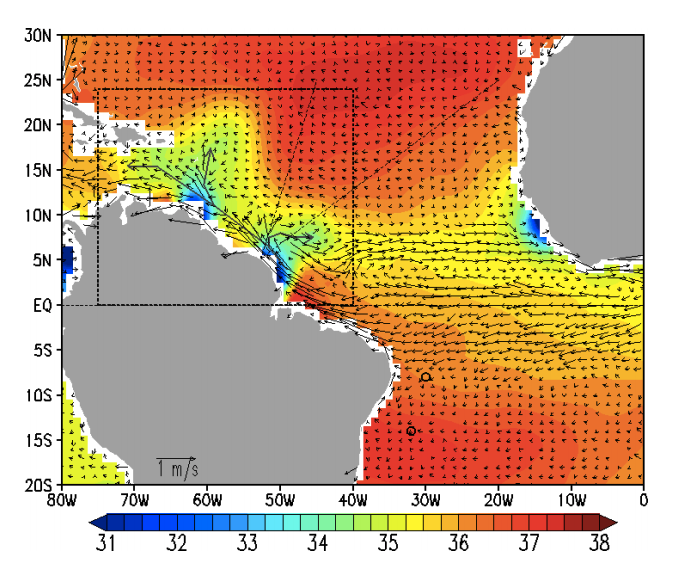
\includegraphics[width=0.5\textwidth]{amazon-diffusion}
        \caption{Salinity is low near the Amazon river mouth as there is a large freshwater input. Salt diffuses as distance from the mouth increases. The rectangle encloses the Amazon plume index region}
\end{figure}

These figures generated with the ECCO data show the northward and eastward advection of salinity.

\begin{figure}[H]
        \centering
        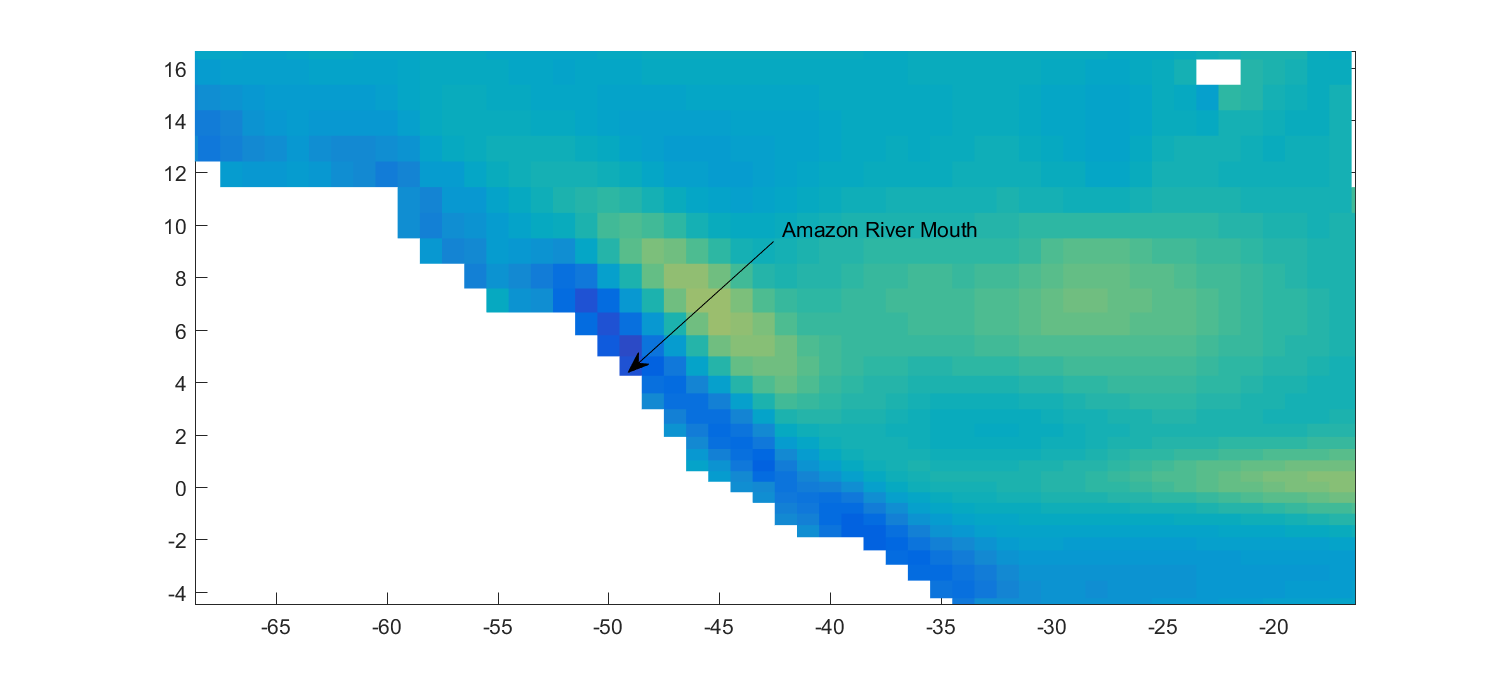
\includegraphics[width=0.5\textwidth]{river-mouth-east-salt}
        \caption{Eastward advection of salt. There is a lot of advection of salt from westward (negative eastward) on the coast of the Amazon. I don't really know why this is...}
\end{figure}

\begin{figure}[H]
        \centering
        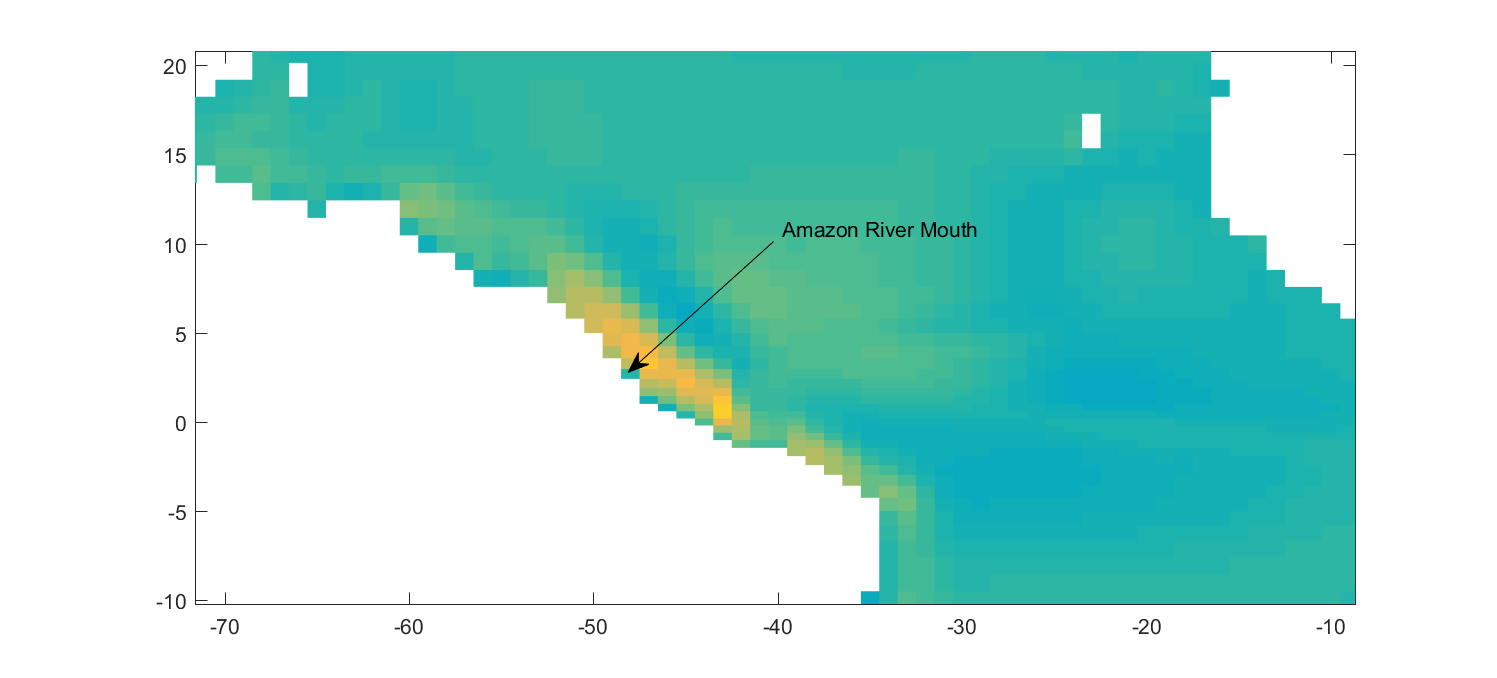
\includegraphics[width=0.5\textwidth]{river-mouth-north-salt}
        \caption{Northward advection of salt near the Amazon. There is a lot of northward salinity advection, perhaps due to the here northward-flowing North Equitorial Current but probably due to other factors that I will hopefully find out about in the papers.}
\end{figure}

\end{document}
